\section{Техническое задание}

\subsection{Основание для разработки}

Основанием для разработки является задание на выпускную квалификационную работу бакалавра «Программно-информационная система для центра повышения квалификации университета».

\subsection{Цель и назначение разработки}

Основной целью работы является разработка и внедрение программно-информационной системы для автоматизации деятельности учебно-методического центра повышения квалификации.

Задачами разработки являются:

\begin{itemize}
	\item создание централизованной базы данных для хранения информации о слушателях, преподавателях, программах обучения, группах и выдаваемых документах;
	\item реализация удобного веб-интерфейса для просмотра, добавления, редактирования и удаления данных;
	\item реализация гибкой системы фильтрации и поиска слушателей по множеству критериев (ФИО, СНИЛС, даты, статусы, программы, кафедры и т.д.);
	\item обеспечение авторизации и разграничения прав доступа (администратор, оператор);
	\item разработка механизма импорта данных из Excel-файлов в формате, предоставляемом заказчиком;
	\item автоматическое формирование статистических отчётов;
	\item создание десктопного приложения для управления серверной частью.
\end{itemize}

\subsection{Требования к функциональности}

Информационная система должна обеспечивать выполнение следующих функций:

\begin{enumerate}
	\item \textbf{Управление данными о слушателях.} Система должна позволять добавлять новых слушателей с заполнением всех необходимых полей (личные данные, обучение, финансы, документ, профессиональные характеристики, предыдущее образование), редактировать и удалять существующие записи, а также просматривать список слушателей в виде таблицы со всеми полями.
	
	\item \textbf{Фильтрация и поиск.} Должна быть реализована возможность текстового поиска по ФИО, СНИЛС и номеру документа. Также необходима фильтрация по полу, возрасту, датам (рождения, начала обучения), наличию ДОТ, множественный выбор статусов слушателей, кафедр, программ и источников финансирования, а также фильтрация по дополнительным полям: педагогический работник, руководитель, область деятельности, квалификация.
	
	\item \textbf{Управление пользователями.} Система должна обеспечивать авторизацию по логину и паролю с разделением прав: администратор имеет полный доступ, оператор — только просмотр. Администратор должен иметь возможность добавлять, редактировать и удалять пользователей.
	
	\item \textbf{Импорт данных.} Должна быть реализована загрузка данных из Excel-файлов (.xlsx) со структурой, соответствующей предоставленному образцу. Перед импортом необходима валидация данных, а по окончании — вывод отчёта с указанием количества обработанных строк и ошибок.
	
	\item \textbf{Статистика и отчётность.} Система должна формировать сводку по слушателям: общее количество, распределение по программам, статусам, источникам финансирования, полу и возрастным группам. Должна быть предусмотрена возможность копирования полученного отчёта в буфер обмена.
	
	\item \textbf{Серверное десктоп-приложение.} Требуется реализовать приложение для запуска и остановки встроенного сервера PostgreSQL и веб-сервера Flask, отображения статуса их работы, а также просмотра логов приложения.
\end{enumerate}

\subsection{Требования к интерфейсу}

Интерфейс информационной системы представляет собой веб-приложение с единым минималистичным стилем оформления, обеспечивающее интуитивно понятную навигацию. Основные элементы интерфейса включают: главную страницу со списком слушателей, панелью фильтров и кнопками управления; страницу добавления и редактирования слушателя с группировкой полей по разделам; форму авторизации; страницу управления пользователями, а также всплывающие окна для просмотра статистики и логов.

На рисунке \ref{fig:index} представлен внешний вид главной страницы веб-приложения.

\begin{figure}[H]
	\centering
	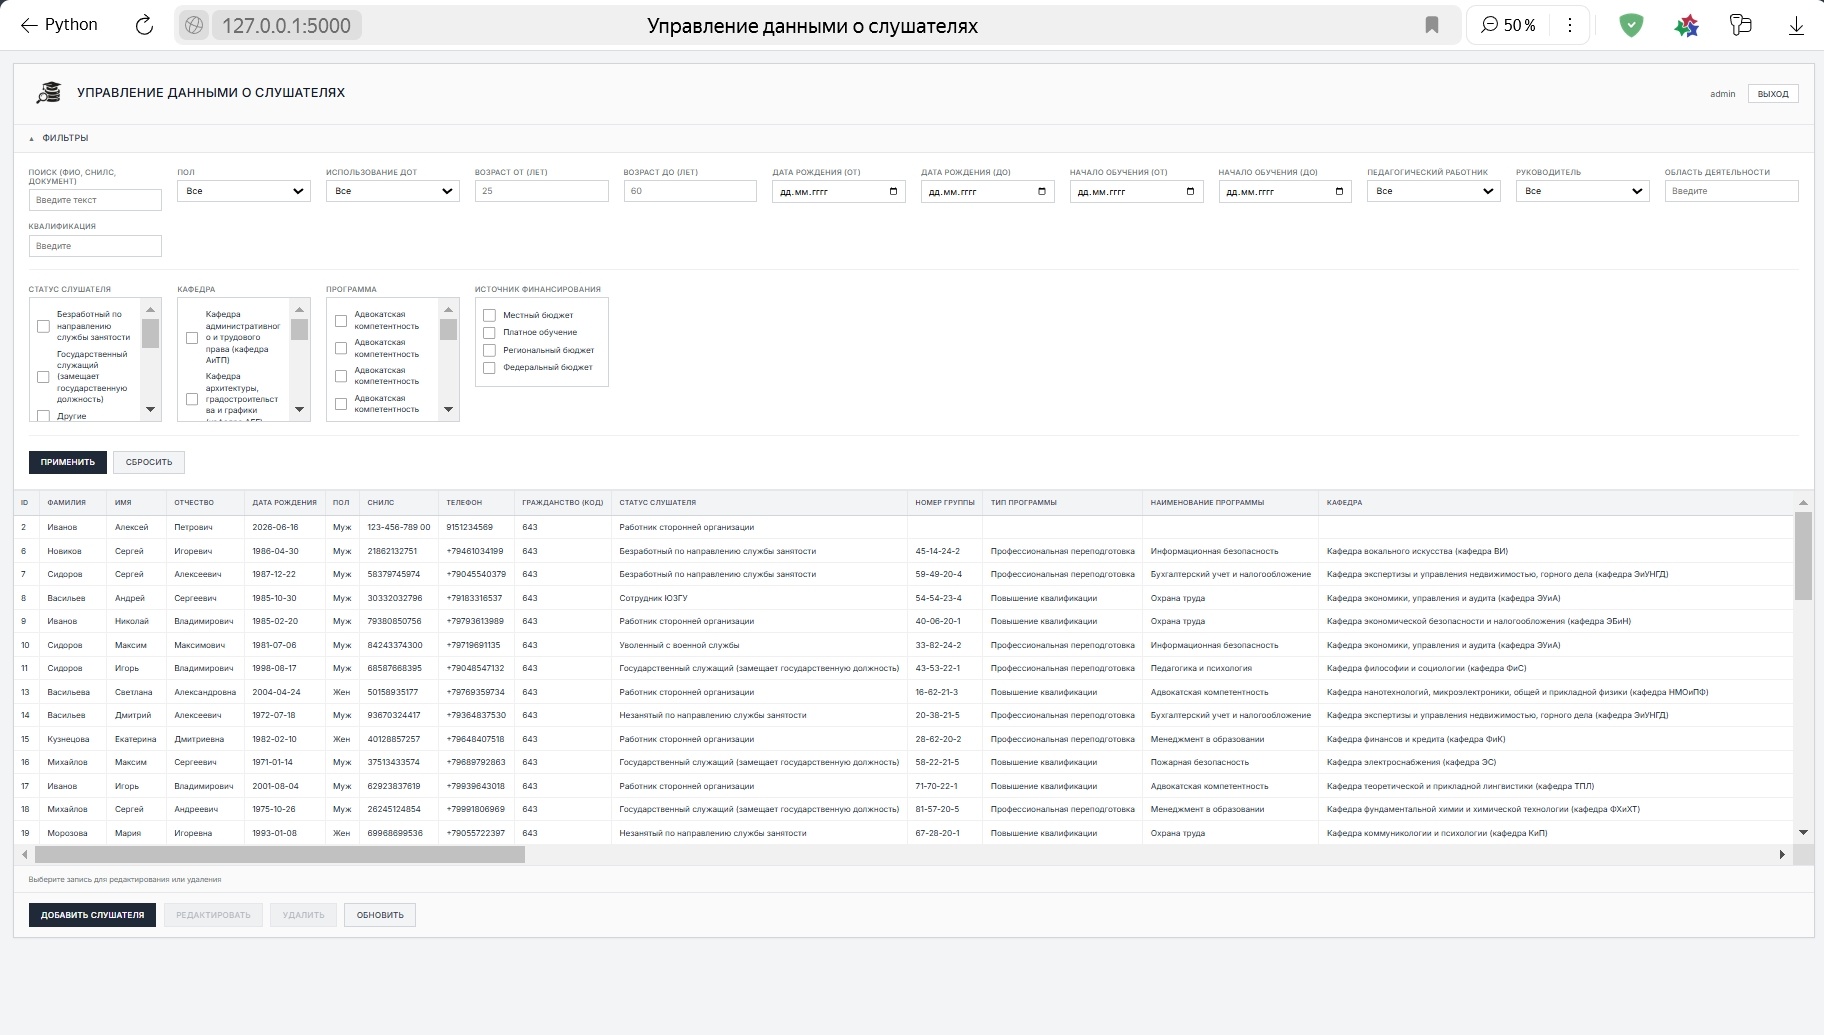
\includegraphics[width=1\linewidth]{index}
	\caption{Главная страница веб-приложения}
	\label{fig:index}
\end{figure}

Как показано на рисунке, главная страница содержит шапку с названием системы, именем текущего пользователя и кнопкой выхода, раскрывающуюся панель для фильтрации данных по различным критериям, таблицу со списком слушателей (ФИО, дата рождения, СНИЛС, статус, программа обучения и др.), а также панель управления с кнопками «Добавить», «Редактировать», «Удалить» и «Обновить».

Вспомогательные окна просмотра журнала событий и статистики показаны на рисунке \ref{fig:logs_stats}.

\begin{figure}[H]
	\centering
	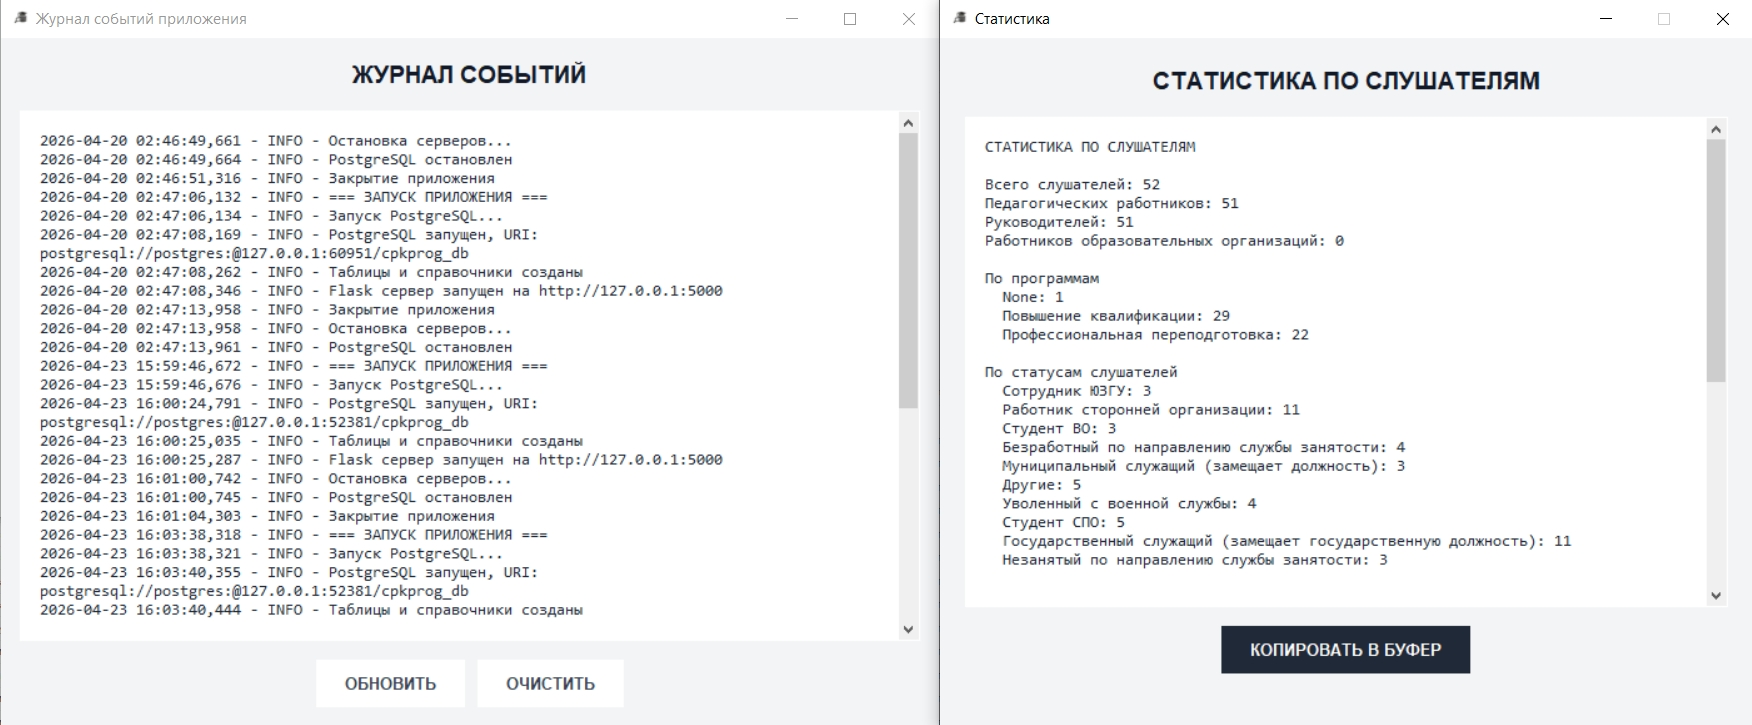
\includegraphics[width=0.9\linewidth]{logs_stats}
	\caption{Окна просмотра журнала событий и статистики}
	\label{fig:logs_stats}
\end{figure}

\subsection{Моделирование вариантов использования}

В системе предусмотрены две роли. Администратор обладает полными правами: просмотр, добавление, редактирование и удаление слушателей, импорт данных, формирование статистики, управление пользователями. Оператор имеет доступ только к просмотру списка слушателей без возможности внесения изменений.

Основные прецеденты (варианты использования) системы:

\begin{enumerate}
	\item Вход в систему.
	\item Просмотр списка слушателей с возможностью фильтрации и поиска.
	\item Добавление нового слушателя.
	\item Редактирование существующего слушателя.
	\item Удаление слушателя.
	\item Импорт данных из Excel-файла.
	\item Просмотр статистики.
	\item Управление пользователями.
	\item Выход из системы.
\end{enumerate}

На рисунке \ref{fig:use_case_web} представлена диаграмма вариантов использования для веб-сайта системы.

\begin{figure}[H]
	\centering
	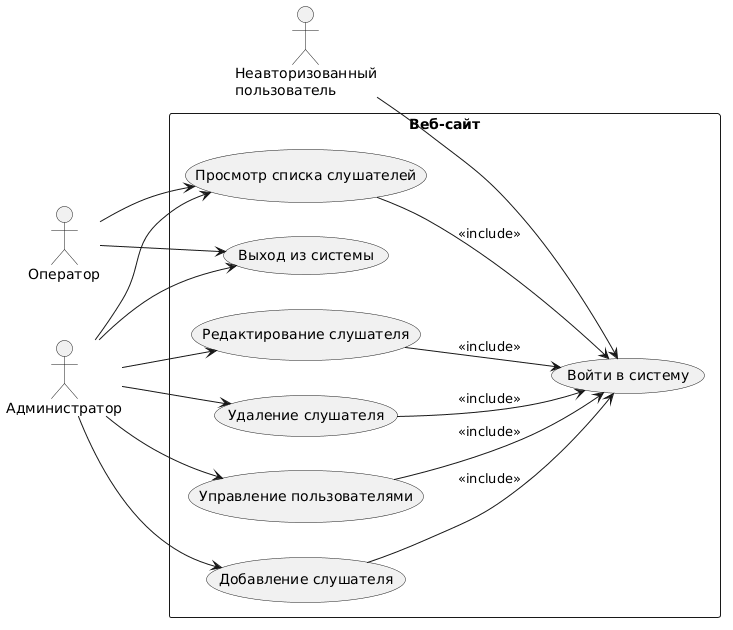
\includegraphics[width=0.9\linewidth]{use_case_web}
	\caption{Диаграмма прецедентов для веб-сайта}
	\label{fig:use_case_web}
\end{figure}

На рисунке \ref{fig:use_case_desk} представлена диаграмма вариантов использования для десктоп-приложения, предназначенного для управления серверной частью.

\begin{figure}[H]
	\centering
	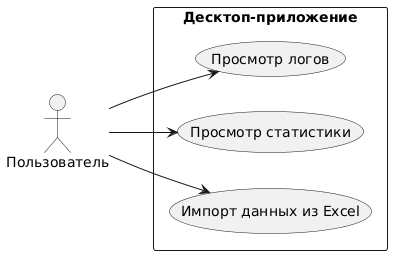
\includegraphics[scale=0.6]{use_case_desk}
	\caption{Диаграмма прецедентов для десктоп-приложения}
	\label{fig:use_case_desk}
\end{figure}

\subsubsection{Вариант использования «Вход в систему»}

\textbf{Заинтересованные лица и их требования:} пользователь (администратор или обычный пользователь) желает получить доступ к функциям системы путём аутентификации по логину и паролю.

\textbf{Предусловие:} пользователь не аутентифицирован в системе; открыта страница входа.

\textbf{Постусловие:} пользователь аутентифицирован, ему предоставлен доступ к функциям системы в соответствии с его уровнем прав (администратор или обычный пользователь).

\textbf{Основной успешный сценарий:}
\begin{enumerate}
	\item Пользователь открывает страницу входа, содержащую поля «Логин» и «Пароль», а также кнопку «Войти».
	\item Пользователь вводит логин и пароль в соответствующие поля.
	\item Пользователь нажимает кнопку «Войти».
	\item Приложение выполняет поиск учётной записи в таблице \texttt{users} базы данных по введённому логину.
	\item Приложение извлекает хеш пароля, сохранённый для данной учётной записи.
	\item Приложение выполняет сравнение введённого пароля с сохранённым хешем с использованием криптографической функции \texttt{check\_password\_hash}.
	\item При совпадении хешей приложение создаёт сессию пользователя и перенаправляет его на главную страницу (список слушателей).
\end{enumerate}

\textbf{Альтернативный сценарий (неверный логин или пароль):}
\begin{enumerate}
	\item На шаге 4 основного сценария учётная запись с введённым логином не найдена, либо на шаге 6 хеши не совпадают.
	\item Приложение отображает сообщение об ошибке: «Неверный логин или пароль».
	\item Пользователь остаётся на странице входа и может повторить попытку.
\end{enumerate}

\subsubsection{Вариант использования «Выход из системы»}

\textbf{Заинтересованные лица и их требования:} аутентифицированный пользователь желает завершить сеанс работы с системой.

\textbf{Предусловие:} пользователь аутентифицирован в системе.

\textbf{Постусловие:} сессия пользователя уничтожена, доступ к защищённым страницам системы заблокирован до повторной аутентификации.

\textbf{Основной успешный сценарий:}
\begin{enumerate}
	\item Пользователь нажимает кнопку «ВЫХОД», расположенную в верхней панели интерфейса.
	\item Приложение вызывает функцию \texttt{logout\_user}, которая уничтожает текущую сессию пользователя.
	\item Приложение перенаправляет пользователя на страницу входа.
\end{enumerate}

\subsubsection{Вариант использования «Добавление нового пользователя»}

\textbf{Заинтересованные лица и их требования:} администратор системы желает создать новую учётную запись для предоставления доступа к системе другому пользователю.

\textbf{Предусловие:} администратор аутентифицирован в системе; открыта страница управления пользователями (\texttt{/admin/users}).

\textbf{Постусловие:} новая учётная запись создана в базе данных; пользователь может войти в систему с указанными логином и паролем.

\textbf{Основной успешный сценарий:}
\begin{enumerate}
	\item Администратор нажимает кнопку «ДОБАВИТЬ ПОЛЬЗОВАТЕЛЯ» на странице управления пользователями.
	\item Приложение отображает форму с полями «Логин», «Пароль» и флажком «Администратор».
	\item Администратор вводит логин и пароль для нового пользователя, при необходимости устанавливает флажок «Администратор».
	\item Администратор нажимает кнопку «СОХРАНИТЬ».
	\item Приложение проверяет, что поля «Логин» и «Пароль» не пусты.
	\item Приложение выполняет запрос к базе данных для проверки уникальности логина.
	\item При отсутствии совпадений приложение вычисляет хеш пароля с использованием функции \texttt{generate\_password\_hash}.
	\item Приложение вставляет новую запись в таблицу \texttt{users} с указанными логином, хешем пароля и признаком администратора.
	\item Приложение отображает сообщение об успешном добавлении пользователя и перенаправляет администратора на страницу списка пользователей.
\end{enumerate}

\textbf{Альтернативный сценарий (логин уже существует):}
\begin{enumerate}
	\item На шаге 6 основного сценария найден пользователь с таким же логином.
	\item Приложение отображает сообщение об ошибке: «Пользователь с таким логином уже существует».
	\item Администратор остаётся на странице формы и может изменить логин.
\end{enumerate}

\textbf{Альтернативный сценарий (пустые обязательные поля):}
\begin{enumerate}
	\item На шаге 5 основного сценария обнаружено, что поле «Логин» или «Пароль» не заполнено.
	\item Приложение отображает сообщение об ошибке: «Логин и пароль обязательны».
	\item Администратор остаётся на странице формы и может заполнить недостающие поля.
\end{enumerate}

\subsubsection{Вариант использования «Редактирование пользователя»}

\textbf{Заинтересованные лица и их требования:} администратор системы желает изменить данные существующей учётной записи (логин, пароль или наличие административных прав).

\textbf{Предусловие:} администратор аутентифицирован в системе; открыта страница управления пользователями (\texttt{/admin/users}); в таблице отображается хотя бы одна учётная запись.

\textbf{Постусловие:} данные учётной записи обновлены в таблице \texttt{users}; при изменении логина или пароля пользователь должен использовать новые учётные данные для входа.

\textbf{Основной успешный сценарий:}
\begin{enumerate}
	\item Администратор нажимает кнопку «РЕДАКТИРОВАТЬ» в строке соответствующего пользователя. Кнопка содержит ссылку вида \texttt{/admin/users/edit/<id>}, где \texttt{<id>} — идентификатор пользователя, полученный из базы данных при формировании таблицы.
	\item Приложение выполняет запрос к базе данных для получения текущих данных пользователя по идентификатору \texttt{<id>}.
	\item Приложение отображает форму редактирования, содержащую поля «Логин» (заполнено текущим значением), «Пароль» (пустое, с подсказкой «оставьте пустым, чтобы не менять»), и флажок «Администратор» (установлен в соответствии с текущим значением).
	\item Администратор изменяет требуемые поля: вводит новый логин, и/или новый пароль, и/или изменяет состояние флажка «Администратор».
	\item Администратор нажимает кнопку «СОХРАНИТЬ».
	\item Приложение проверяет, что поле «Логин» не пусто.
	\item Приложение выполняет запрос к базе данных для проверки уникальности нового логина (исключая текущего пользователя с идентификатором \texttt{<id>}).
	\item Если введён новый пароль, приложение вычисляет его хеш с использованием функции \texttt{generate\_password\_hash}; если поле пароля оставлено пустым, существующий хеш сохраняется без изменений.
	\item Приложение выполняет обновление записи в таблице \texttt{users}.
	\item Приложение отображает сообщение «Пользователь обновлён» и перенаправляет администратора на страницу списка пользователей.
\end{enumerate}

\textbf{Альтернативный сценарий (логин занят другим пользователем):}
\begin{enumerate}
	\item На шаге 7 основного сценария обнаружено, что введённый логин уже принадлежит другому пользователю.
	\item Приложение отображает сообщение об ошибке: «Пользователь с таким логином уже существует».
	\item Администратор остаётся на странице формы и может изменить логин на другой. Введённые данные, кроме логина, сохраняются в форме.
\end{enumerate}

\textbf{Альтернативный сценарий (пользователь не найден):}
\begin{enumerate}
	\item На шаге 2 основного сценария запрос к базе данных не возвращает результат (запись была удалена другим администратором между загрузкой страницы и нажатием кнопки, либо идентификатор был изменён вручную в адресной строке).
	\item Приложение возвращает HTTP-ответ с кодом 404 (Not Found) и отображает сообщение «Пользователь не найден».
\end{enumerate}

\subsubsection{Вариант использования «Удаление пользователя»}

\textbf{Заинтересованные лица и их требования:} администратор системы желает удалить учётную запись пользователя, которому больше не требуется доступ к системе.

\textbf{Предусловие:} администратор аутентифицирован в системе; открыта страница управления пользователями (\texttt{/admin/users}); существует удаляемая учётная запись.

\textbf{Постусловие:} учётная запись удалена из таблицы \texttt{users}; пользователь больше не может войти в систему.

\textbf{Основной успешный сценарий:}
\begin{enumerate}
	\item Администратор нажимает кнопку «УДАЛИТЬ» в строке соответствующего пользователя.
	\item Приложение отображает диалоговое окно подтверждения с сообщением «Удалить пользователя?».
	\item Администратор подтверждает удаление нажатием кнопки «ОК».
	\item Приложение проверяет, что идентификатор удаляемого пользователя не совпадает с идентификатором текущего администратора.
	\item Приложение выполняет запрос \texttt{DELETE FROM users WHERE id = \%s} к базе данных.
	\item Приложение отображает сообщение «Пользователь удалён» и обновляет список пользователей.
\end{enumerate}

\textbf{Альтернативный сценарий (попытка удаления самого себя):}
\begin{enumerate}
	\item На шаге 4 основного сценария обнаружено, что администратор пытается удалить собственную учётную запись.
	\item Приложение отображает сообщение об ошибке: «Нельзя удалить самого себя».
	\item Учётная запись не удаляется, администратор остаётся на странице списка пользователей.
\end{enumerate}

\subsubsection{Вариант использования «Просмотр списка слушателей»}

\textbf{Заинтересованные лица и их требования:} пользователь желает ознакомиться с перечнем слушателей, содержащихся в базе данных системы.

\textbf{Предусловие:} пользователь аутентифицирован в системе.

\textbf{Постусловие:} на экране отображена таблица со списком слушателей.

\textbf{Основной успешный сценарий:}
\begin{enumerate}
	\item Пользователь открывает главную страницу приложения.
	\item Приложение запрашивает из базы данных список всех слушателей, включая связанные данные (группа, программа, кафедра, документ, финансирование и т.\,д.).
	\item Приложение запрашивает из базы данных значения справочников (статусы, кафедры, программы, источники финансирования) для заполнения панели фильтров.
	\item Приложение формирует HTML-страницу, содержащую таблицу со слушателями и панель фильтров.
	\item Браузер отображает страницу. Таблица имеет фиксированную высоту с вертикальной прокруткой, заголовки колонок зафиксированы и остаются видимыми при прокрутке.
\end{enumerate}

\subsubsection{Вариант использования «Добавление нового слушателя»}

\textbf{Заинтересованные лица и их требования:} пользователь желает внести в базу данных информацию о новом слушателе.

\textbf{Предусловие:} пользователь аутентифицирован в системе.

\textbf{Постусловие:} новый слушатель и все связанные с ним данные сохранены в базе данных; слушатель отображается в общем списке.

\textbf{Основной успешный сценарий:}
\begin{enumerate}
	\item Пользователь нажимает кнопку «ДОБАВИТЬ СЛУШАТЕЛЯ» на главной странице.
	\item Приложение отображает форму добавления слушателя, содержащую пять тематических разделов: «Личные данные», «Обучение», «Финансы», «Документ о квалификации», «Профессиональные характеристики», «Предыдущее образование». Форма включает текстовые поля, выпадающие списки, поля выбора дат и числовые поля.
	\item Пользователь заполняет поля формы.
	\item Пользователь нажимает кнопку «СОХРАНИТЬ».
	\item Приложение выполняет валидацию введённых данных.
	\item При успешной валидации приложение сохраняет данные слушателя и всех связанных записей в базе данных.
	\item Приложение перенаправляет пользователя на главную страницу, где отображается обновлённый список слушателей.
\end{enumerate}

\textbf{Альтернативный сценарий (ошибка валидации):}
\begin{enumerate}
	\item На шаге 5 основного сценария валидация обнаруживает ошибки.
	\item Приложение отображает форму с сообщением об ошибке и сохраняет все ранее введённые пользователем данные в полях формы, чтобы пользователю не требовалось заполнять их заново.
\end{enumerate}

\subsubsection{Вариант использования «Редактирование данных слушателя»}

\textbf{Заинтересованные лица и их требования:} пользователь желает изменить данные ранее добавленного слушателя.

\textbf{Предусловие:} пользователь аутентифицирован в системе; слушатель с указанным идентификатором существует в базе данных.

\textbf{Постусловие:} данные слушателя и всех связанных записей обновлены в базе данных.

\textbf{Основной успешный сценарий:}
\begin{enumerate}
	\item Пользователь на главной странице выбирает слушателя, щёлкнув по соответствующей строке таблицы. Выбранная строка подсвечивается.
	\item Кнопка «РЕДАКТИРОВАТЬ», ранее неактивная, становится активной.
	\item Пользователь нажимает кнопку «РЕДАКТИРОВАТЬ».
	\item Приложение загружает из базы данных текущие данные выбранного слушателя.
	\item Приложение отображает форму редактирования, идентичную форме добавления, с полями, предзаполненными текущими значениями.
	\item Пользователь изменяет требуемые поля.
	\item Пользователь нажимает кнопку «СОХРАНИТЬ ИЗМЕНЕНИЯ».
	\item Приложение выполняет валидацию изменённых данных.
	\item При успешной валидации приложение обновляет данные слушателя и всех связанных записей в базе данных.
	\item Приложение перенаправляет пользователя на главную страницу с обновлённым списком.
\end{enumerate}

\textbf{Альтернативный сценарий (слушатель не найден):}
\begin{enumerate}
	\item На шаге 4 основного сценария запись с указанным идентификатором не обнаружена.
	\item Приложение отображает сообщение «Студент не найден».
\end{enumerate}

\textbf{Альтернативный сценарий (ошибка валидации при редактировании):}
\begin{enumerate}
	\item На шаге 8 основного сценария валидация обнаруживает ошибки.
	\item Приложение отображает форму редактирования с сообщением об ошибке; некорректные значения сохраняются в полях формы, остальные поля содержат актуальные данные из базы данных.
\end{enumerate}

\subsubsection{Вариант использования «Удаление слушателя»}

\textbf{Заинтересованные лица и их требования:} пользователь желает удалить запись о слушателе из базы данных.

\textbf{Предусловие:} пользователь аутентифицирован в системе; на главной странице отображается список слушателей; выбран конкретный слушатель.

\textbf{Постусловие:} запись о слушателе и все связанные с ней данные удалены из базы данных; слушатель больше не отображается в списке.

\textbf{Основной успешный сценарий:}
\begin{enumerate}
	\item Пользователь на главной странице выбирает слушателя, щёлкнув по соответствующей строке таблицы. Выбранная строка подсвечивается.
	\item Кнопка «УДАЛИТЬ», ранее неактивная, становится активной.
	\item Пользователь нажимает кнопку «УДАЛИТЬ».
	\item Приложение отображает диалоговое окно подтверждения с сообщением «Удалить слушателя?».
	\item Пользователь подтверждает удаление.
	\item Приложение выполняет удаление записи слушателя из базы данных.
	\item Приложение перенаправляет пользователя на главную страницу с обновлённым списком слушателей.
\end{enumerate}

\textbf{Альтернативный сценарий (отмена удаления):}
\begin{enumerate}
	\item На шаге 4 основного сценария пользователь отказывается от удаления.
	\item Никаких изменений в базе данных не производится, страница остаётся в текущем состоянии.
\end{enumerate}

\subsubsection{Вариант использования «Установка фильтров для отбора слушателей»}

\textbf{Заинтересованные лица и их требования:} пользователь желает сократить объём отображаемых данных, отобрав слушателей по одному или нескольким критериям.

\textbf{Предусловие:} пользователь аутентифицирован в системе; открыта главная страница со списком слушателей.

\textbf{Постусловие:} таблица слушателей обновлена и содержит только записи, удовлетворяющие заданным критериям. Параметры фильтрации сохранены в URL страницы.

\textbf{Основной успешный сценарий:}
\begin{enumerate}
	\item Пользователь раскрывает панель фильтров, нажав на заголовок «ФИЛЬТРЫ». При первом открытии страницы панель уже раскрыта.
	\item Пользователь устанавливает один или несколько критериев фильтрации. Панель фильтров предоставляет следующие типы элементов ввода:
	\begin{itemize}
		\item текстовое поле для поиска по подстроке (поиск по ФИО, СНИЛС, номеру документа);
		\item выпадающие списки для выбора одного значения из предопределённого набора (пол, использование ДОТ, педагогический работник, руководитель);
		\item числовые поля и поля выбора дат для задания диапазонов (возраст, дата рождения, дата начала обучения);
		\item текстовые поля для поиска по справочным значениям (область деятельности, квалификация);
		\item списки с флажками для множественного выбора (статусы слушателей, кафедры, программы, источники финансирования).
	\end{itemize}
	\item Пользователь нажимает кнопку «ПРИМЕНИТЬ».
	\item Приложение формирует запрос к базе данных с учётом всех заданных критериев. Различные критерии объединяются логической операцией «И», при множественном выборе внутри одного критерия — операцией «ИЛИ».
	\item Приложение получает отфильтрованный список слушателей и обновляет содержимое таблицы.
	\item Параметры фильтрации сохраняются в URL страницы, что позволяет обновить страницу без потери настроек.
\end{enumerate}

\subsubsection{Вариант использования «Сброс фильтров»}

\textbf{Заинтересованные лица и их требования:} пользователь желает отменить все установленные ранее критерии фильтрации и вернуться к просмотру полного списка слушателей.

\textbf{Предусловие:} пользователь аутентифицирован в системе; открыта главная страница; применён хотя бы один критерий фильтрации.

\textbf{Постусловие:} все фильтры сброшены; таблица отображает полный список слушателей.

\textbf{Основной успешный сценарий:}
\begin{enumerate}
	\item Пользователь нажимает кнопку «СБРОСИТЬ», расположенную рядом с кнопкой «ПРИМЕНИТЬ» на панели фильтров.
	\item Приложение выполняет переход на главную страницу без параметров фильтрации в URL (маршрут \texttt{/}).
	\item Приложение загружает полный список слушателей из базы данных.
	\item Таблица обновляется, отображая всех слушателей. Все элементы панели фильтров возвращаются в исходное состояние (пустые поля ввода, выпадающие списки в значении «Все», все флажки сняты).
\end{enumerate}

\subsubsection{Вариант использования «Импорт слушателей из Excel-файла»}

\textbf{Заинтересованные лица и их требования:} пользователь желает загрузить в базу данных множество записей о слушателях из заранее подготовленного файла в формате Excel (XLSX).

\textbf{Предусловие:} пользователь находится в графическом интерфейсе программы; база данных запущена.

\textbf{Постусловие:} корректные записи из файла добавлены в базу данных; ошибочные записи пропущены; информация о результатах импорта отображена пользователю; ошибки записаны в лог-файл.

\textbf{Основной успешный сценарий:}
\begin{enumerate}
	\item Пользователь нажимает кнопку «ЗАГРУЗИТЬ ИЗ EXCEL» в главном окне программы.
	\item Приложение открывает стандартный диалог выбора файла с фильтром по расширению \texttt{.xlsx}.
	\item Пользователь выбирает файл и подтверждает выбор.
	\item Приложение загружает справочники из базы данных для последующего сопоставления текстовых значений с идентификаторами.
	\item Приложение читает содержимое Excel-файла. Все ячейки интерпретируются как строки.
	\item Приложение выполняет сопоставление заголовков столбцов файла с внутренними ключами системы (например, заголовок «Фамилия получателя» сопоставляется с ключом \texttt{last\_name}).
	\item Для каждой строки файла приложение формирует словарь данных, аналогичный данным формы веб-интерфейса, и преобразует текстовые значения справочных полей в соответствующие идентификаторы.
	\item Для каждой строки выполняется валидация данных по тем же правилам, что и при добавлении через веб-интерфейс.
	\item При успешной валидации данные вставляются в базу данных.
	\item При обнаружении ошибок валидации или ошибок базы данных строка пропускается, информация об ошибке записывается в лог-файл \texttt{import\_errors.log}.
	\item По завершении обработки всех строк приложение отображает окно с результатами импорта: общее количество строк в файле, количество успешно добавленных записей, количество ошибок, текст последней ошибки.
\end{enumerate}

\textbf{Альтернативный сценарий (файл не выбран):}
\begin{enumerate}
	\item На шаге 2 основного сценария пользователь закрывает диалог выбора файла, не выбрав файл.
	\item Импорт не производится, приложение остаётся в исходном состоянии.
\end{enumerate}

\textbf{Альтернативный сценарий (ошибка чтения файла):}
\begin{enumerate}
	\item На шаге 5 основного сценария возникает ошибка при чтении файла (файл повреждён, не является Excel-файлом или имеет неверную структуру).
	\item Приложение отображает сообщение об ошибке. Импорт прекращается.
\end{enumerate}

\subsubsection{Вариант использования «Просмотр статистики по слушателям»}

\textbf{Заинтересованные лица и их требования:} пользователь желает получить сводную аналитическую информацию о слушателях, содержащихся в базе данных.

\textbf{Предусловие:} база данных запущена; пользователь находится в графическом интерфейсе программы.

\textbf{Постусловие:} на экране отображено окно со статистическим отчётом.

\textbf{Основной успешный сценарий:}
\begin{enumerate}
	\item Пользователь нажимает кнопку «СТАТИСТИКА» в главном окне программы.
	\item Приложение выполняет серию запросов к базе данных для сбора статистических показателей:
	\begin{itemize}
		\item общее количество слушателей;
		\item количество педагогических работников;
		\item количество руководителей;
		\item количество работников образовательных организаций;
		\item распределение слушателей по типам программ;
		\item распределение по статусам слушателей;
		\item распределение по источникам финансирования;
		\item распределение по полу;
		\item распределение по возрастным группам;
		\item количество студентов высшего и среднего профессионального образования.
	\end{itemize}
	\item Приложение формирует текстовый отчёт, содержащий все собранные показатели.
	\item Приложение отображает отчёт в отдельном окне. Текст отчёта доступен для просмотра с вертикальной прокруткой.
\end{enumerate}

\textbf{Альтернативный сценарий (база данных не запущена):}
\begin{enumerate}
	\item На шаге 1 основного сценария кнопка «СТАТИСТИКА» недоступна, так как её состояние зависит от статуса сервера.
	\item Пользователь не может инициировать просмотр статистики до запуска базы данных.
\end{enumerate}

\textbf{Альтернативный сценарий (ошибка получения статистики):}
\begin{enumerate}
	\item На шаге 2 основного сценария возникает ошибка при выполнении запросов к базе данных.
	\item Приложение отображает окно с сообщением об ошибке.
\end{enumerate}

\subsubsection{Вариант использования «Копирование статистики в буфер обмена»}

\textbf{Заинтересованные лица и их требования:} пользователь желает скопировать текст статистического отчёта для последующей вставки в другой документ.

\textbf{Предусловие:} открыто окно со статистическим отчётом.

\textbf{Постусловие:} текст отчёта помещён в буфер обмена операционной системы.

\textbf{Основной успешный сценарий:}
\begin{enumerate}
	\item Пользователь нажимает кнопку «КОПИРОВАТЬ В БУФЕР» в окне статистики.
	\item Приложение копирует полный текст статистического отчёта в буфер обмена.
	\item Приложение отображает кратковременное подтверждение «Скопировано!» рядом с кнопкой.
\end{enumerate}

\subsubsection{Вариант использования «Просмотр журнала событий»}

\textbf{Заинтересованные лица и их требования:} пользователь (администратор системы) желает ознакомиться с журналом событий приложения для диагностики ошибок или отслеживания истории запусков и остановок.

\textbf{Предусловие:} программа запущена.

\textbf{Постусловие:} на экране отображено отдельное окно с содержимым файла журнала событий.

\textbf{Основной успешный сценарий:}
\begin{enumerate}
	\item Пользователь нажимает кнопку «ЖУРНАЛ СОБЫТИЙ» в главном окне программы.
	\item Приложение открывает отдельное окно, содержащее текстовое поле с прокруткой.
	\item Приложение читает содержимое файла \texttt{app.log} и отображает его в текстовом поле.
	\item Каждая запись журнала содержит временную метку, уровень важности и текст сообщения.
\end{enumerate}

\textbf{Дополнительные возможности:}

\textbf{Обновление журнала.} Пользователь может нажать кнопку «ОБНОВИТЬ» в окне журнала, чтобы загрузить актуальное содержимое файла. Это позволяет отслеживать события в реальном времени, не закрывая окно.

\textbf{Очистка журнала.} Пользователь может нажать кнопку «ОЧИСТИТЬ» для удаления всех записей из файла журнала. После очистки содержимое окна обновляется и становится пустым.

\subsection{Требования к надёжности}

Система должна обеспечивать надёжное хранение и обработку данных при различных режимах работы.

\textbf{Целостность данных.} База данных PostgreSQL поддерживает механизм транзакций, гарантирующий, что операции добавления, редактирования и удаления данных либо выполняются полностью, либо откатываются в исходное состояние при возникновении ошибки. Это исключает появление частично сохранённых или противоречивых данных.

\textbf{Устойчивость к сбоям.} При аварийном завершении работы сервера (например, при отключении электропитания) PostgreSQL автоматически выполняет восстановление базы данных при следующем запуске. Все успешно сохранённые транзакции восстанавливаются, незавершённые — откатываются.

\textbf{Контроль целостности на уровне приложения.} На уровне веб-приложения реализована валидация вводимых данных: проверка форматов дат, СНИЛС, телефона, кода гражданства, стоимости обучения и других полей. Это предотвращает попадание некорректных данных в базу.

\textbf{Логирование ошибок.} Все критические ошибки и исключения, возникающие при работе системы, записываются в файл журнала (app.log). Лог содержит временную метку, тип ошибки и описание причины, что облегчает диагностику неполадок.

\textbf{Резервное копирование.} Данные системы хранятся в файлах базы данных PostgreSQL (папка pgdata). Для обеспечения сохранности информации администратор может выполнить резервное копирование простым копированием данной папки или через штатные средства PostgreSQL (pg\_dump). Восстановление данных осуществляется обратным копированием.

\subsection{Требования к информационной безопасности}

Система должна обеспечивать защиту данных от несанкционированного доступа и разграничение прав пользователей.

\textbf{Авторизация.} Доступ к веб-приложению осуществляется только после ввода логина и пароля. Форма авторизации является единственной точкой входа для неавторизованных пользователей.

\textbf{Хранение паролей.} Пароли пользователей не хранятся в базе данных в открытом виде. Для их хранения используется хеширование. При авторизации введённый пароль сверяется с хешем, хранящимся в базе.

\textbf{Разграничение прав доступа.} В системе предусмотрены две роли. Администратор обладает полными правами, в то время как оператор имеет доступ только к просмотру списка слушателей без возможности внесения изменений. После успешной авторизации пользователь получает права, соответствующие его роли. Проверка прав выполняется на серверной стороне перед выполнением любого действия, что исключает возможность обхода ограничений через клиентский код.

\textbf{Защита от несанкционированного доступа.} Десктоп-приложение не требует авторизации, так как предполагается, что доступ к нему имеют только уполномоченные сотрудники. Серверная часть принимает подключения только на локальном интерфейсе (127.0.0.1), что ограничивает доступ к системе из внешней сети.

\textbf{Защита от SQL-инъекций.} Все запросы к базе данных выполняются с использованием параметризованных SQL-запросов (библиотека psycopg2), что исключает возможность внедрения произвольного SQL-кода через пользовательский ввод.

\subsection{Требования к программной и технической совместимости}

Система должна функционировать в типовой офисной среде и не предъявлять завышенных требований к оборудованию.

\textbf{Операционная система.} Собранное приложение является автономным и работает под управлением операционной системы Windows. Возможна работа под управлением Linux или macOS при условии сборки приложения на соответствующей платформе (исполняемый файл, собранный в среде Windows, не может быть запущен в других операционных системах). Сборка выполняется с использованием PyInstaller и включает все необходимые компоненты: интерпретатор Python, библиотеки и бинарные файлы PostgreSQL.

\textbf{Аппаратные требования:}
\begin{itemize}
	\item процессор: 2 ГГц и выше;
	\item оперативная память: 4 ГБ и более;
	\item свободное дисковое пространство: 500 МБ для программы, дополнительно — для хранения базы данных.
\end{itemize}

\textbf{Программное обеспечение.} Для работы веб-интерфейса необходим любой современный браузер: Google Chrome, Mozilla Firefox, Microsoft Edge. Десктоп-приложение не требует установки дополнительного программного обеспечения — PostgreSQL и Flask встраиваются непосредственно в приложение с использованием библиотеки pgembed, а интерпретатор Python не требуется, так как он упакован в исполняемый файл.

\textbf{Сетевые требования.} Веб-сервер слушает порт 5000 на всех сетевых интерфейсах (0.0.0.0), что позволяет подключаться к системе не только с локального компьютера, но и с других устройств в локальной сети.

\textbf{Требования к сопровождающей документации.} Система поставляется в виде исполняемого файла и не требует установки. Пользователю достаточно запустить файл, нажать кнопку «Запустить сервер» и дождаться открытия браузера. Для администратора предусмотрен файл журнала событий и возможность просмотра логов через интерфейс десктоп-приложения.

\subsection{Требования к оформлению документации}

Разработка программной документации и программного изделия должна производиться согласно ГОСТ 19.102-77 и ГОСТ 34.601-90. Единая система программной документации.